% Chapter 3

\chapter{Tecniche di animazione} % Design

\label{Chapter3} % For referencing this chapter elsewhere, use \ref{ChapterX}

Animare significa ``muovere" un modello, altrimenti statico, nel tempo. Questi movimenti sono definiti attraverso delle trasformazioni geometriche (traslazione, rotazione e scalatura).
Di seguito vengono riportate alcune tecniche di animazione 3D, spiegandone le metodologie, i pregi, i difetti e il contesto in cui possono venire utilizzate.


\section{Rappresentazioni di rotazione}
Iniziamo spigando come si possa rappresentare una rotazione. Alcuni di questi concetti sono validi anche per altre trasformazioni, tuttavia prenderò in considerazione solo le rotazioni in quanto sono uno degli aspetti principali nella realizzazione di animazioni --- in particolare di animazioni 3D --- e anche uno dei più complessi.


\subsection{Angolo-asse}
Questo tipo di rappresentazione è senza dubbio la più semplice.
Utilizza 4 valori: 3 per specificare l'asse, ed 1 per l'angolo. In questo modo, con una singola rotazione, è possibile raggiungere qualsiasi orientamento dell'oggetto che si sta ruotando. Così come esiste sempre una linea retta che collega due punti nello spazio, si può pensare ad una rotazione angolo-asse come una singola rotazione che collega due orientamenti.

Questa rappresentazione, è ottima per rotazioni di giunture con un solo DOF, mentre il suo comportamento può diventare contro intuitivo per giunture con più di un DOF. Inoltre anche la rappresentazione dell'asse attraverso 3 componenti numeriche non risulta di facile comprensione.

\subsection{Euleriana}

\begin{figure}[]
\centering
\begin{subfigure}{.5\textwidth}
  \centering
  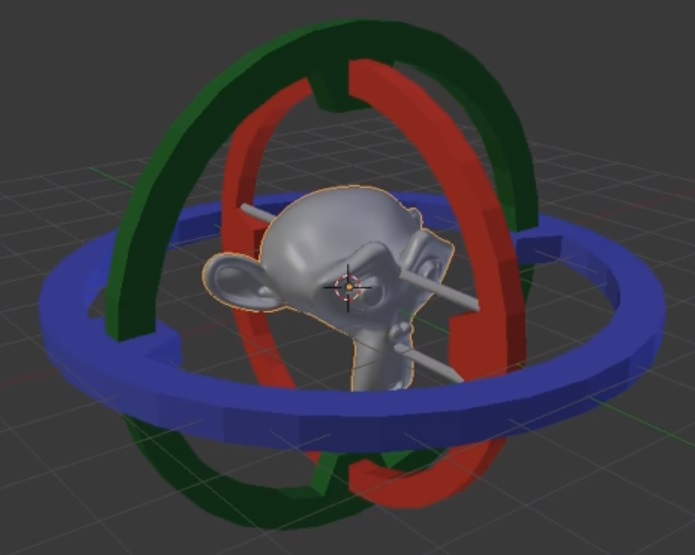
\includegraphics[width=.9\linewidth]{Figures/euler-1.jpg}
  \caption{Posizione neutra}
  \label{fig:sub1}
\end{subfigure}%
\begin{subfigure}{.5\textwidth}
  \centering
  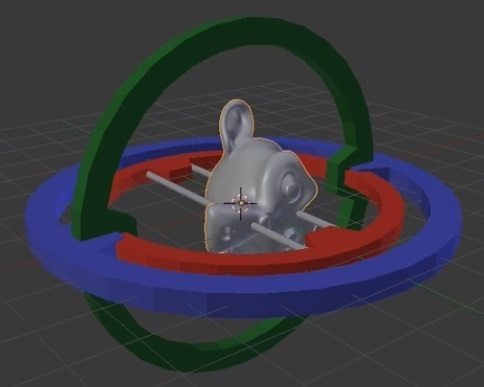
\includegraphics[width=.9\linewidth]{Figures/euler-2.jpg}
  \caption{Gimbal lock, l'asse X e Z sono allineati}
  \label{fig:sub2}
\end{subfigure}
\decoRule
\caption[Rotazione euleriana]{Rappresentazione di rotazione euleriana attraverso un giroscopio a tre assi}
\label{fig:euler1}
\end{figure}

La più intuitiva di tutte: utilizza 3 assi di rotazione (X, Y, Z) ed il funzionamento è analogo a quello di un giroscopio. ogni asse offre un DOF, quindi sono possibili rotazioni con 3 DOF. Tuttavia sono necessarie due accortezze: 
\begin{enumerate}
    \item ordine degli assi;
    \item gimbal lock problem.
\end{enumerate}
L'ordine degli assi è decisivo, in quanto quello più interno dipende dalla rotazione di quelli esterni. Di conseguenza ruotando gli assi in un ordine diverso da quello specificato porta a risultati diversi da quello atteso. In più, interpolazioni tra diverse orientazioni possono a loro volta risultare differenti da ciò che ci si sarebbe aspettato.

Il problema del gimbal lock \parencite{anticz16}, in italiano blocco cardanico, sorge dall'allineamento di due assi: quello più interno e quello più esterno. Ne deriva che ruotano uno di questi 2 assi si ottiene la stessa rotazione, perdendo quindi un DOF.
È quindi importante scegliere l'ordine degli assi in maniera tale che il primo e il terzo non risultino mai allineati.





\subsection{Quaternaria}

\subsection{Matriciale}
Quest'ultima è la rappresentazione ottimale, in quanto permette di rappresentare anche traslazioni, scalature e altre trasformazioni come \emph{shear}. È, infatti, la rappresentazione che blender utilizza internamente \parencite{blendApi, nat2012rig} poiché quella che offre la maggior flessibilità. L'unico difetto è che, come la rappresentazione quaternaria, non mantiene l'informazione sul percorso della rotazione. Infatti è ancora più simile a una delta-rotazione (i.e. differenza di orientamento), rispetto alla rappresentazione quaternaria poiché copre una rotazione di soli 360\textdegree, rispetto ai 720\textdegree\ delle quaternarie. 


